\section{Experiments}
\label{sec:experiments}
In this section, we present a systematic large-scale experimental evaluation of our algorithm.
\subsection{Experimental setting}
\label{subsec:expsetting}
\paragraph{Dataset} 
We use $9$ real-world datasets from various sources, detailed in Appendix~\ref{appendix:datasets}. Each dataset contains no fewer than $50,000$ data points, ranges from $3$ to $22$ dimensions and is linked to a binary classification or regression task, which we use to evaluate the downstream error. For these evaluations, we allocate $80\%$ of the data as private data $D$ and use the remaining $20\%$ for test data $D_{test}$.  We discretize every dimension containing real values or integer values exceeding a range of $32$ into $32$ equally-sized bins.

\paragraph{Privacy Budget} We use $\epsilon =2.5$ and $\delta =10^{-5}$ as default choices. According to the National Institute of Standards and Technology (NIST), $\epsilon$ values below $5$ can be considered as strong privacy protection and real-world applications commonly use values above $2.5$ \citep{NIST-diff-privacy}. 


\paragraph{Metrics} We evaluate the statistical and downstream task performance of our algorithm with the following standard metrics for DP data  synthesis:
\begin{itemize}


    \item[1.] \textit{downstream error:} The classification/regression test error, i.e., the $0$-$1$ (resp. mean squared) error, of gradient boosting trained on the synthesized data $\dpdata$  and evaluated on the (non-privatized) test dataset $D_{test}$. 
    \item[2.] \textit{covariance error:} The Frobenius norm of the differences of the centered covariance matrices of $\embed(D) $ and $\embed(\dpdata)$ divided by the Frobenius norm of the centered covariance matrix of $\embed(\dpdata)$. Since the embedding just rescales the (discretized) variables, this is equivalent to computing the covariance matrix error of the normalized data, up to a constant.
\end{itemize}

Moreover, we use the relative average over $J =200$  query differences between $\dpdata$ and $D$
    \begin{equation}
    \label{eq:countquery}
      \frac{ \frac{1}{J}\sum_j\vert \text{query}_j(\dpdata) - \text{query}_j(D)\vert }{  \frac{1}{J}\sum_j \text{query}_j(D)}.
    \end{equation}
    

We instantiate the query difference 
for two commonly used queries (see e.g., \cite{vietri2022private}):
    \begin{itemize}
        \item[3.] \textit{count. queries:} $3$-sparse counting queries 
with $\text{query}_j(D)= \text{count}_j(D) = \frac{1}{n} \sum_i 
\mathbbm{1}[x_i \in \mathcal A_j] $  with  $A_j$ the full hypercube $\forall l: A_j^l = {1, \dots, k_l}$ except for $3$ random dimensions where the $A_j^l$ is an interval with uniformly drawn lower bound and subsequently drawn upper bound. We use rejection sampling to ensure that at least 5\% and at most 95\% of the samples of the original dataset fall in this interval for every $j$. 
\item[4.] \textit{thresh. queries:}
    %The relative average difference of 
    $3$-sparse linear thresholding queries 
    %as in Equation \eqref{eq:countquery}
with $\text{query}_j(D)=\text{thrs}_j(D) = \frac{1}{n} \sum_i  
\mathbbm{1}_{\langle x_i, \theta \rangle + b_j >0} $; $\theta$ is a random $3$-sparse direction and $b_j$ is uniformly drawn from the interval $[\min_{x \in D} \langle x, \theta \rangle,\max_{x \in D} \langle x, \theta \rangle]$.
 \end{itemize}

 Finally, we compute the average sliced Wasserstein distance and the total variation distance. The former is approximately minimized by PrivPGD while the latter by existing marginal-based approaches (e.g., \citep{aim,mst}):
\begin{itemize}
    \item[5.] \emph{average $\swd_1$ dist.:}  
    The average $\swd_1$ distance over all $2$-Way marginals between the embedded empirical probability measures  of the original dataset $D$  and the DP dataset $\dpdata$;
    $\mu_S[D], \mu_S[\dpdata] \in  \mathcal P(\embed(\domain)_S)$: 
    % \fy{not sure that was really helpful here, and to me created parser error more than clarified or move to after the equation}
    \begin{equation}
        {d \choose 2}^{-1} \sum_{S \subset [d]; \vert S \vert =2 } \swd_1 \left( \mu_S[D] , \mu_S[\dpdata]\right) 
    \end{equation}
        \item[6.] \emph{average TV dist.:} The average total variation distance $\text{TV}$ over all $2$-Way marginals between the original dataset $D$ and the DP dataset $\dpdata$
        %$\marginal{S}[D], \marginal{S}[\dpdata] \in  \mathcal P(\domain_S)$:
    \begin{equation}
        {d \choose 2}^{-1} \sum_{S \subset [d]; \vert S \vert =2 } \text{TV}\left( \marginal{S}[D], \marginal{S}[\dpdata]\right) 
    \end{equation}
\end{itemize}

 




  \paragraph{Implementation of PrivPGD}
 We implement PrivPGD using \textit{PyTorch} on a GPU and use the same hyperparameters for all experiments. We select all $2$-Way marginals and use the Gaussian mechanism to construct DP-copies of them  (step 2 in Algorithm~\ref{alg:mainalgo}). We then generate a dataset by running PrivPGD (Algorithm~\ref{alg:pgd}) with  $100k$ particles. 


 
 For the \emph{projection step} (Section~\ref{sec:projection}), we use $200$ MC random projections to approximate the $\swd_1$ distance. We construct the finite measure $ \hat \omega_{S, \mathbb P}$ by running gradient descent for $1750$ iterations using \text{Adam} with an initial learning rate of $0.1$ and a linear learning rate scheduler with step size $100$ and multiplicative factor $0.8$. As initialization, we use the probability measure obtained when setting all negative weights of $\hat \omega_{S}$ to zero and subsequently normalize the positive finite measure. 

 
In the \emph{optimization step} (Section~\ref{subsec:optimization}), we  approximate the $\swd^2_2$ using $N_{\text{MC}} =10$ projections. We minimize the objective in \Cref{eq:loss_gd} by running gradient descent for $1000$ epochs (where in every epoch every marginal is seen exactly once) using an initial learning rate of $0.1$ and a linear learning rate scheduler with step size $50$ and multiplicative factor $0.75$. We divide $\mathcal S$ into mini-batches of size $5$ and randomly set $80\%$ of the gradient entries to zero. We use \textit{Sparse Adam} from the $\textit{PyTorch}$ package.

\paragraph{Implementation of the metrics} We use the implementation from \textit{scikit-learn}~\citep{sklearn_api} for Gradient Boosting using the standard hyperparameters. Since discretization is a separate problem on its own, we use the discretized dataset in all experiments. 

\subsection{Algorithms for benchmarking}
\label{sec:algorithms}
We benchmark PrivPGD against a number of baselines including representative PGM-based and query-based methods. The PGM-based methods include MST \citep{mst} and AIM \cite{aim}. For AIM, we choose all $2$-Way marginals as workload. The following query-based algorithms include Private GSD \citep{pmlr-v202-liu23ag}, RAP \cite{aydore2021differentially} and GEM \citep{liu2021iterative}, where we choose all 2-Way marginals as queries. 

\emph{Implementation of AIM and MST.} We implement MST and AIM using the code provided by the authors\footnote{ \url{https://github.com/ryan112358/private-pgm}.}. We choose the initial learning rate to be $1.0$ and run mirror descent for $3000$ iterations. We fix the hyperparameters for all experiments. Moreover, we slightly modify the code for MST and AIM by increasing the sensitivity used in the Gaussian \citep{gauss_mechanism} and exponential mechanisms \citep{mcsherry2007mechanism} to give accurate privacy guarantees for the differential privacy model from Definition~\ref{eq:defdp}. 
We refer to \citep{aim} for an overview of both mechanisms in the context of DP data release. 

\emph{Implementation of query-based algorithms.} We use the one-shot version of Private GSD from the paper with an elite size of 2 and early stopping, and tune the number of generations $G \in \{200k, 500k\}$, the mutation and crossover populations $P_{mut} = P_{cross} \in \{50, 100, 150, 200, 500\}$, and the number of synthesized data points $m \in \{2k, 100k\}$. For GEM, we keep the default hyperparameters, tuning the number of iterations $T \in \{3, 10, 30, 50, 100, 150, 200\}$ and the model architecture $layers_{MLP} \in \{[512, 512, 1024], [128, 256]\}$. 
For RAP, we also keep the default hyperparameters and tune  $T \in \{3, 10, 30, 50, 100, 150, 200\}$, the learning rate $lr \in \{0.0001, 0.001, 0.03\}$ and $m \in \{2k, 500k\}$. This hyperparameter optimization includes the configurations considered by \citet{pmlr-v202-liu23ag}. All methods are implemented using their official versions, with hyperparameters fine-tuned for each dataset. GEM and RAP could not be run for the ACS Employment dataset due to exceeding our memory constraint of 20 GB.

 \begin{figure*}[t!]


    \centering
  \begin{subfigure}{\linewidth}
        \centering

\includegraphics[width=0.9\textwidth]{figures/exp12legend_plot.pdf}
    \end{subfigure}
    \includeBenchFigures{figures/plots_datasets/eps_2.5/}
        \centering
    \caption{
    \small 
    Comparison of PrivPGD with all $2$-Way marginals against state-of-the-art methods based on metrics from Section~\ref{subsec:expsetting}: 1) downstream error, 2) covariance error, 3) count. queries error, and 4) thresh. queries error, across 9 tabular datasets. For each method, we plot the $\log_2$ ratio of the errors, using PrivPGD's average error as the denominator, and report the mean and standard deviation over 5 runs. We cut at a log ratio of $y=4$ (dashed line) and list all methods exceeding this threshold above this line in order. We set $\epsilon = 2.5$ and $\delta = 10^{-5}$.
}    
    \label{fig:comp}
    \vspace{-0.2in}
\end{figure*}

  \subsection{Comparison with baselines}
\label{sec:exp_priv_marginals}


We now present how the performance of PrivPGD compares against the state-of-the-art algorithms for DP data synthesis. Figure~\ref{fig:comp} illustrates the relative performance of PrivPGD compared to other methods, using metrics from Section~\ref{subsec:expsetting}. PrivPGD consistently ranks as either the best or the second-best in most metrics and datasets, with a few exceptions such as the covariance error in the ACS Public Coverage dataset.

\paragraph{Comparison with PGM}
PrivPGD systematically outperforms both variants of PGM, which are the state-of-the-art for marginal-based tabular data synthesis, often by a significant margin. Specifically, it is better than PGM+MST in covariance and query errors across datasets, except for thresholding query errors in the Diabetes dataset, and performs at least as well as PGM+AIM, usually surpassing it, with the notable exception of thresholding query errors in the ACS Mobility dataset. For downstream tasks, PrivPGD performs comparably to PGM+AIM and consistently better than PGM+MST.


\paragraph{Comparison with query-based algorithms}
Furthermore, PrivPGD is also the preferred method in most scenarios when compared to query-based approaches, especially against GEM and RAP. While Private GSD provides competitive performance and occasionally surpasses PrivPGD – for instance, in the ACS Public Coverage dataset – PrivPGD usually emerges as the best-performing method. On many datasets it significantly outperforms Private GSD in all metrics, as exemplified by the Taxi, Black Friday, and ACS Traveltime datasets.


\paragraph{$\swd_1$ and TV distance} Finally, Figure~\ref{fig:comp_sw_tv_2.5} illustrates a noticeable performance gap between PrivPGD and other methods when comparing the average sliced Wasserstein distance and the total variation distance. PrivPGD effectively minimizes the former, while state-of-the-art methods like PGM primarily target the latter. Our experiments demonstrate the advantage of minimizing a geometry-aware loss function like the sliced Wasserstein distance over the total variation distance.




\begin{figure*}
    \centering
    \begin{subfigure}{\linewidth}
        \centering
        
\includegraphics[width=0.9\textwidth]{figures/exp12legend_plot.pdf}
    \end{subfigure}
    \includeDistFigures{figures/plots_distances/eps_2.5/}
        \centering
        \caption{\small Comparison of average $\swd_1$ distance (left) and average TV distance (right) for PrivPGD against state-of-the-art methods across 9 tabular datasets. Similar to Figure~\ref{fig:comp}, we report the mean and standard deviation (5 runs) of the $\log_2$ ratio of errors. We set $\epsilon = 2.5$ and $\delta = 10^{-5}$.}

        \label{fig:comp_sw_tv_2.5}
\end{figure*}
\subsection{Enforcing additional domain-specific constraints}
\label{sec:domainspecific_exp}

\begin{wrapfigure}{r}{0.52\textwidth}
\vspace{-0.3in}
    \centering
        \begin{subfigure}{\linewidth}
        \centering

\includegraphics[width=\textwidth]{figures/plots_constraint/exp3_legend.pdf}
    \end{subfigure}
    \begin{subfigure}{.45\linewidth}
        \centering
        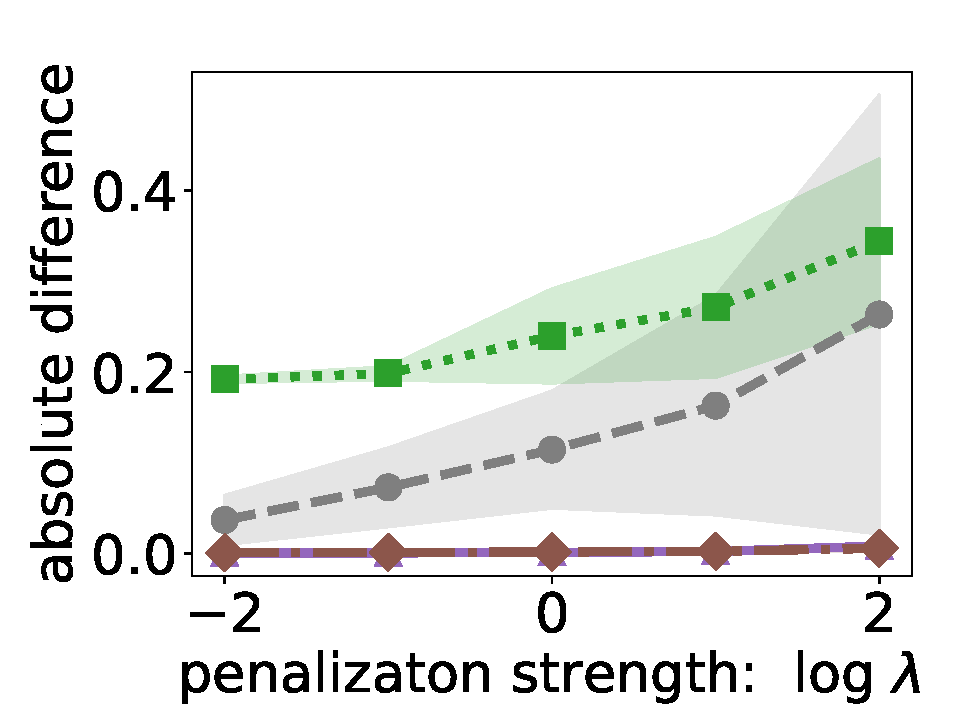
\includegraphics[width=\textwidth]{figures/plots_constraint/exp3_acs_income_CA_2018_default_32+thresholding_1.pdf}
        \caption{ACS Income}
    \end{subfigure}%
    \begin{subfigure}{.45\linewidth}
        \centering
        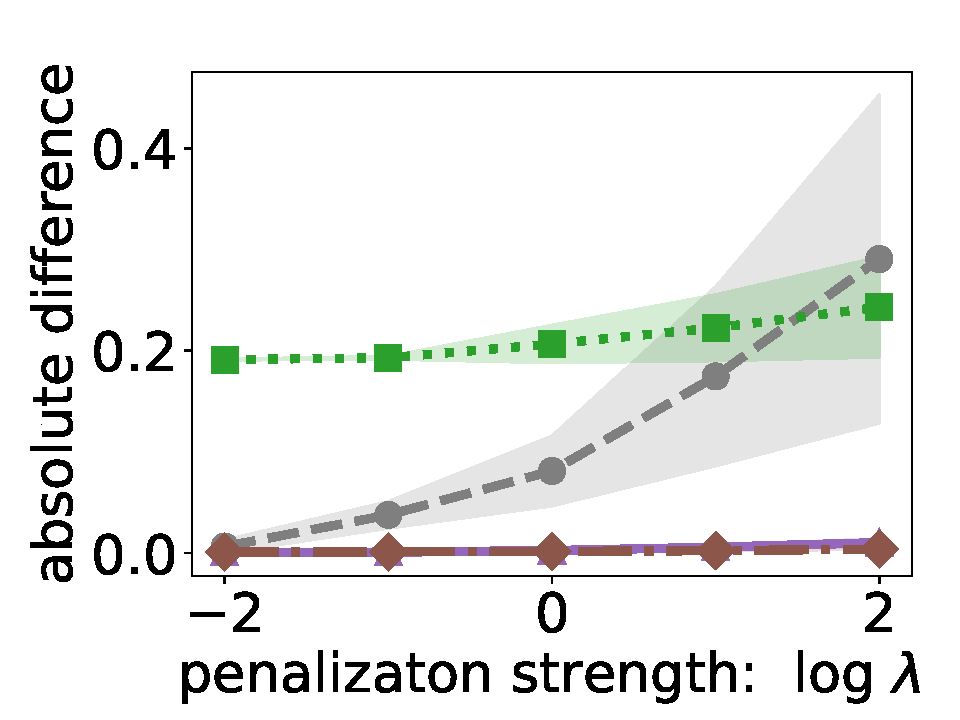
\includegraphics[width=\textwidth]{figures/plots_constraint/exp3_acs_employment_CA_2018_default_32+thresholding_1.pdf}
        \caption{ACS Employment}
    \end{subfigure}
    \caption{\small  The absolute error of the domain-specific query (larger is better), the downstream classification error (smaller is better), and the absolute error over counting and thresholding queries (smaller is better), i.e., only the numerator in ~\Eqref{eq:countquery}, as a function of the log regularization strength $\lambda$. We plot the curves for (a) the Income and (b) the Employment dataset. }
    \label{fig:3}
    \vspace{-0.3in}
\end{wrapfigure}

Section \ref{sec:exp_priv_marginals} shows that PrivPGD constructs a private dataset that successfully preserves the relevant statistics of the original dataset. 
However, while differential privacy protects individual information, many applications require the protection of specific population-level statistics, i.e., one would like specific statistics from the DP-dataset $\dpdata$ to have a large \emph{mismatch} with statistics from the original dataset $D$. 
This goal is in contrast to the utility loss that tries to match certain statistics of the original dataset.
One example is census data, where it might be desirable to hide religious or sexual orientations at the subpopulation level to prevent potential discriminatory misuse of the data. Another example is the publication of rental and house sale prices, where exposing certain correlations could lead to speculative abuses in specific locales.

We now demonstrate how PrivPGD, while constructing a high-quality dataset,
% preserving the metrics from above
 allows the protection of statistics on a population level. As an example, we consider maximizing the distance of a single linear (non-sparse) thresholding query $    \text{thrs}_{\embed}(\particles) = \frac{1}{m} \sum_i 
\mathbbm{1}_{\langle \particles_i, \theta \rangle + b >0}$ defined directly in the embedding space. We approximate this query using a differentiable sigmoid approximation and define $\hat \queryloss(Z) = \frac{1}{c + (\triangle(Z))^2}$ where $\triangle(Z)$ is the difference to a DP-estimate of the original data. We refer to the Appendix~\ref{appendix:details_domain} for details.


 We plot in Figure~\ref{fig:3} the absolute thresholding error as a function of the regularization strength $\lambda$. While the query is well approximated if no (or only little) regularization is used, we see how increasing the regularization strength increasingly protects these statistics, as the domain-specific counting query on $\dpdata$ deviates strongly from the one on the original data $D$. 
We further plot the downstream error and the absolute errors over random counting and thresholding queries (only the numerator in~\Cref{eq:countquery}). We observe that, even for larger regularization penalties, these statistics are still preserved, comparable to the unregularized case. 



\section{Conclusion and future work}


We introduced PrivPGD, a novel generation method for marginal-based private data synthesis. Our approach leverages particle gradient descent, combined with techniques from optimal transport, resulting in improved performance in a large number of settings, enhanced scalability for handling numerous marginals and larger datasets, and increased flexibility for accommodating domain-specific constraints compared to existing methods.

% PrivPGD typically outperforms PGM-based methods and state-of-the-art query-based algorithms like GEM and RAP in our experimental evaluations. However, it is occasionally surpassed by Private GSD. While PrivPGD generally performs better, it is not clear in which specific settings one method outshines the other. 
Future work could develop regularization penalties that promote an inductive bias in PrivPGD towards more favorable solutions, similar to the maximum entropy bias in PGM. Additionally, exploring the design of domain-specific differentiable constraints and applying our method in practical scenarios presents an exciting avenue for future research.


\section{Acknowledgements}

KD was supported by the ETH AI Center and the ETH Foundations of Data Science. JA was supported by the ETH AI Center. We thank Aram Alexandre Pooladin and Guillaume Wang for insightful discussions.



